%%%%%%%%%%%%%%%%%%%%%%%%%%%%%%%%%%%%%%%%%
% University/School Laboratory Report
% LaTeX Template
% Version 3.1 (25/3/14)
%
% This template has been downloaded from:
% http://www.LaTeXTemplates.com
%
% Original author:
% Linux and Unix Users Group at Virginia Tech Wiki 
% (https://vtluug.org/wiki/Example_LaTeX_chem_lab_report)
%
% License:
% CC BY-NC-SA 3.0 (http://creativecommons.org/licenses/by-nc-sa/3.0/)
%
%%%%%%%%%%%%%%%%%%%%%%%%%%%%%%%%%%%%%%%%%

%----------------------------------------------------------------------------------------
%	PACKAGES AND DOCUMENT CONFIGURATIONS
%----------------------------------------------------------------------------------------

\documentclass{article}

\usepackage{graphicx} % Required for the inclusion of images
\graphicspath{ {images/} } % path for images
\usepackage{subcaption} % placing multiple images on one by one in a line
\usepackage{wrapfig} % placing an image along with text in a line
\usepackage{natbib} % Required to change bibliography style to APA
\usepackage{amsmath} % Required for some math elements 
\usepackage{enumerate} % use enumarated lists

\setlength\parindent{0pt} % Removes all indentation from paragraphs

\renewcommand{\labelenumi}{\alph{enumi}.} % Make numbering in the enumerate environment by letter rather than number (e.g. section 6)

\usepackage{times} % Uncomment to use the Times New Roman font

%----------------------------------------------------------------------------------------
%	DOCUMENT INFORMATION
%----------------------------------------------------------------------------------------

\title{Lab Project: Computer Graphics \\ Building a basic ray tracer \\ SS2017} % Title

\author{Haralambi \textsc{Todorov}} % Author name

\date{\today} % Date for the report

\begin{document}

\maketitle % Insert the title, author and date

\begin{center}
\begin{tabular}{l r}
Advisor: & Prof. Dr.-Ing. Matthias Teschner % Instructor/supervisor
\end{tabular}
\end{center}

% If you wish to include an abstract, uncomment the lines below
% \begin{abstract}
% Abstract text
% \end{abstract}

%----------------------------------------------------------------------------------------
%	SECTION 1
%----------------------------------------------------------------------------------------

\section{Introduction}
\label{sec:intro}
The main objective of the \textit{Lab project: Computer Graphics} was to make the author familiar with the basic concepts of a ray tracer by implementing one. This lab report aims to present the gathered knowledge.

% explain the structure of the current lab report
\subsection{Report overview}
The report is split into five chapters with, each explaining a certain part of the implemented ray tracer. The ordering of the chapters tries to follow the implementation order the author followed during the project. 

\vspace*{\baselineskip}

Current chapter (\ref{sec:intro}) is an introductory one giving details about the organisation of this report, motivation about why is ray tracing an important rendering technique and where does it find application nowadays, along with some information on the roots of ray tracing, the basic idea of the ray tracing algorithm and some implementation notes regarding the accompanying ray tracer.

\vspace*{\baselineskip}

Chapter (\ref{sec:isects}) deals with one of the fundamental parts of a ray tracer, the ray-object intersection test. It starts with the geometric definition of a half-line (ray), goes on with the different type of geometries the ray tracer supports (spheres, triangles, axis-aligned boxes and triangulated meshes) and how the half-line intersects with these geometries.

\vspace*{\baselineskip}

Chapter (\ref{sec:cameras}) is concerned with how the camera and the image plane are modelled in the ray tracer. It explains the virtual pinhole camera model, how the image plane is mapped within the 3D scene and the two supported camera projections - orthographic and perspective along with their configurable parameters. The chapter goes on with how rays are shot from the image plane and how one can reduce aliasing artefacts by using half-jittered sampling technique. It finishes with the use of gamma correction to enhance the visual appearance of the generated images. 

\vspace*{\baselineskip}

Chapter (\ref{sec:shading}) deals with the visual appearance of objects rendered in a scene. It begins by explaining how light sources are modeled, goes on with the concept behind the Phong illumination model and the physical motivation behind its components, how shadows are ray traced and lastly, it presents reflective and refractive materials and how these types of materials are ray traced.

\vspace*{\baselineskip}

Chapter (\ref{sec:transform}) deals with transformations, explaining the motivation behind the use of homogeneous notation, the different type of supported transformations on objects, light sources and cameras and why the inverse view transformation is useful in a ray tracer.

\vspace*{\baselineskip}

Chapter (\ref{sec:accel}) is concerned with how one can reduce the computation time per generated image by introducing acceleration structures. Firstly, it explains the concept behind axis-aligned bounding boxes and the benefits they bring, followed by a more advanced acceleration method, the uniform grid.

% why should one bother to implement a ray tracer
\subsection{Why is ray tracing important}
Ray tracing is one of the rendering techniques capable of producing images with a high degree of visual realism. It can naturally incorporate physically motivated visual effects such as reflections, refractions, caustics, soft shadows and others. This advantage makes the technique very attractive to movie and commercial studios, automotive industry (see figure \ref{fig:audi}), as well as architectural design studios (see figure \ref{fig:arch}) to simulate realistic illumination.  

\begin{figure}[h]
	\centering
	
	% show car image
	\begin{subfigure}{0.5\textwidth}
		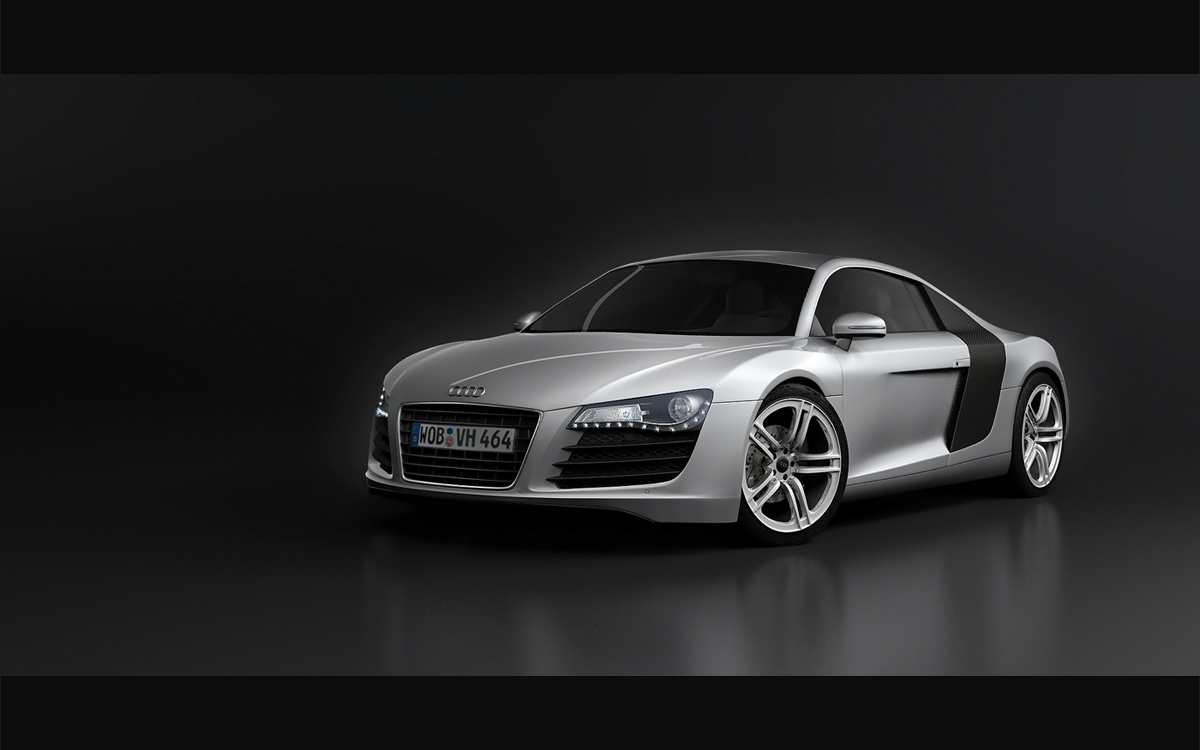
\includegraphics[width=0.9\textwidth]{audi}
		\caption{"Another R8" by Filip Sadlon \\ rendered using Blender Render}
		\label{fig:audi}
	\end{subfigure}%
	\hfill
	\begin{subfigure}{0.5\textwidth}
		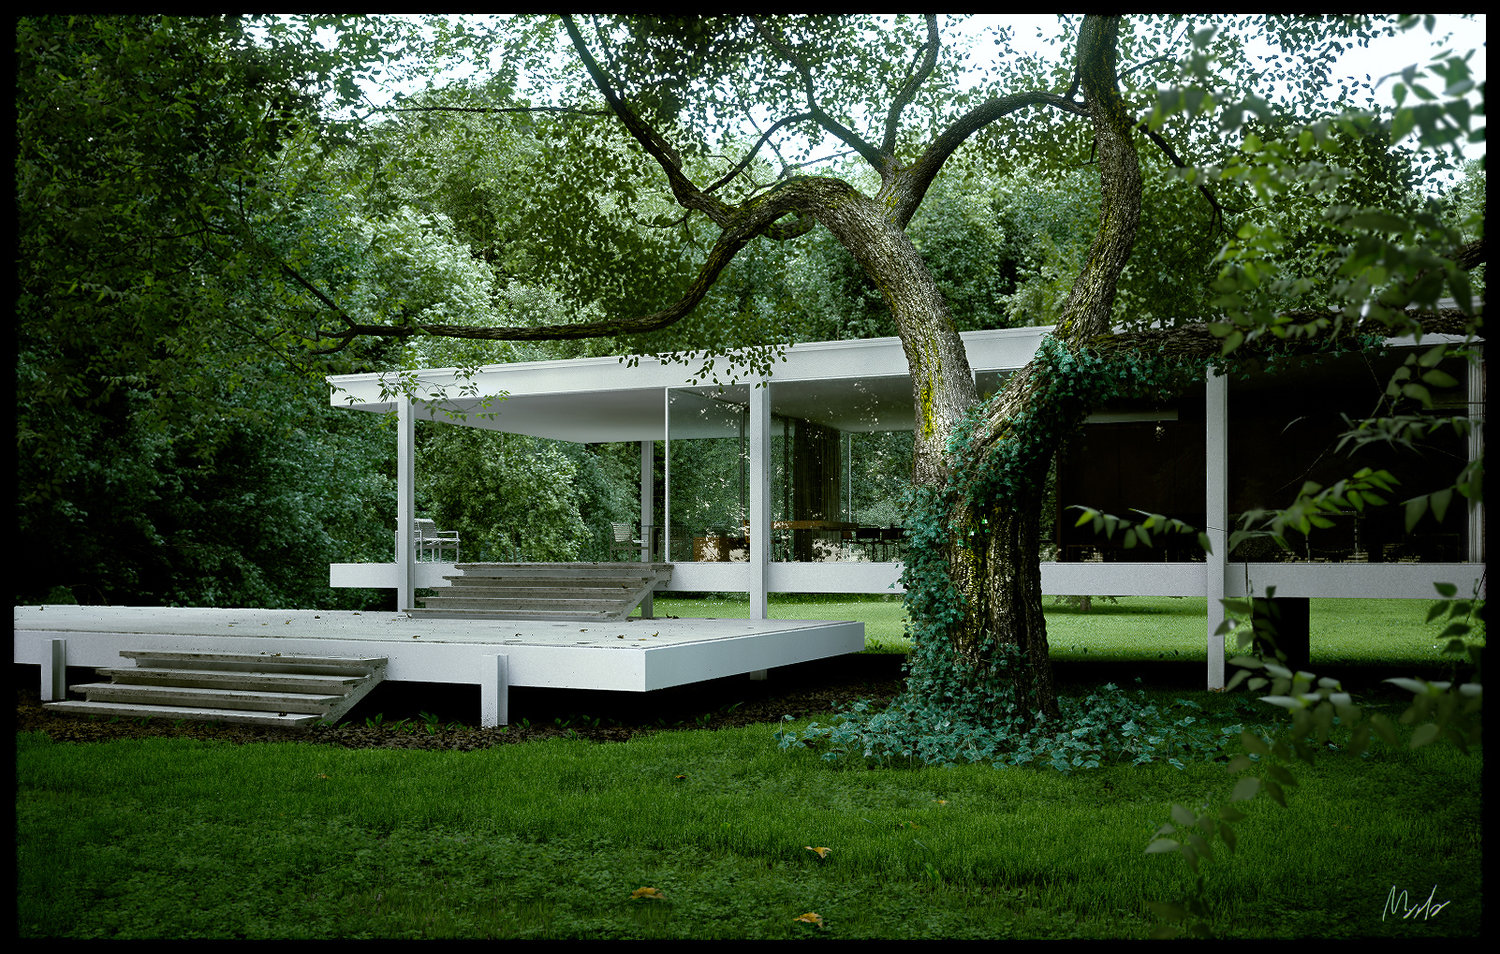
\includegraphics[width=0.9\textwidth]{archi_render}
		\caption{"Mies Van Der Rohe Farnsworth House" by Alessandro Prodan using Mental Ray}
		\label{fig:arch}
	\end{subfigure}
	
	\caption{Ray tracing used for visualisations by different industries}
\end{figure}

Although one can produce very stunning imagery with a ray tracing based render engine, this  comes at a great computational cost, e.g.\ a frame from a recent computer generated Pixar's movie takes between three and eight hours to render. \cite{pixarRentime} \\
Despite great computation times, major animation studios seem nowadays to be fond of ray tracing and switch to ray tracing from scanline-based rendering approaches, such as "REYES", which have been proved stable and fast over the years to ray tracing. \cite{pixarSwitch} That points to the demands in the entertainment industry for more physically accurate imagery, but also pushes the boundaries of research in ray tracing and its computational efficiency. \cite{disneyHyperion}

% some history behind ray tracing
\subsection{The roots of ray tracing}
The first ray tracing algorithm was introduced by Arthur Appel in 1968 \cite{appel}, whose idea was to shoot rays from the eye (camera), one per pixel, and find the closest object blocking the path of that ray. Using the material properties and the effect of the lights in the scene, this algorithm can determine the shading of objects. \\
The next notable contribution in ray tracing was made by Turner Whitted in 1979 \cite{whitted}, who introduced a technique to compute shadows, as well as the idea of recursive ray tracing to handle reflective and refractive materials. (see figure \ref{fig:whitted_example}).  

Other major contributions in the scene of ray tracing were made by Robert Cook in 1984 \cite{cook} and James Kajiya in 1986 \citep{kajiya}, introducing distributed ray tracing and the Rendering equation respectively. Because the accompanying ray tracer does not make extensive use of these concepts, they won't be discussed in detail.

% show whitted like image
\begin{figure}[h]
	\centering
    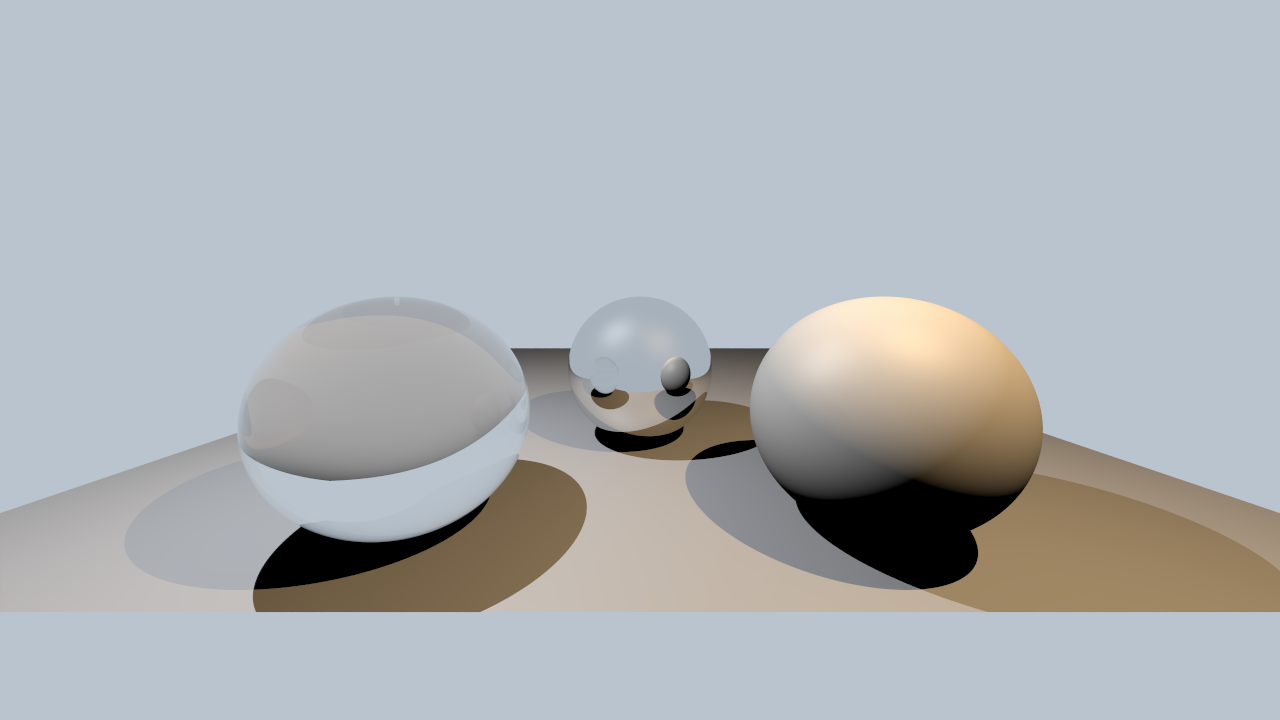
\includegraphics[width=0.8\textwidth]{whitted_example}
    \caption{A Whitted-like scene with reflective (back) and refractive (front left) spheres rendered in the accompanying ray tracer}
    \label{fig:whitted_example}
\end{figure}

% basic ray tracing algorithm concept
\subsection{Basics of the ray tracing algorithm}
For the following explanation we make the assumption we have a camera with perspective projection. The algorithm then works by tracing a path from an imaginary eye (camera) through each pixel in a virtual image plane (in front of the camera) and calculating the radiance of the object visible through it.

Typically, each ray must be tested for intersection with some subset of all the objects in the scene. Once the nearest object has been identified, the algorithm will estimate the incoming light at the point of intersection, examine the material properties of the object, and combine this information to calculate the final color of the pixel (see figure \ref{fig:concept}). 

% show image depicting basic ray tracing algorithm
\begin{figure}[h]
	\centering
    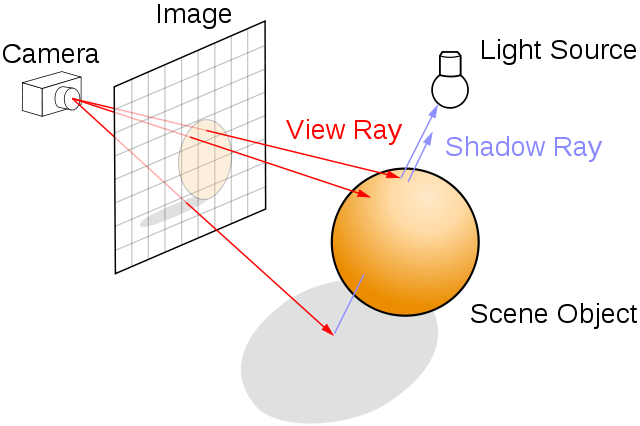
\includegraphics[width=0.6\textwidth]{ray_trace_algo}
	\caption{Image depicting the concept behind the ray tracing algorithm. Wikipedia}
    \label{fig:concept}
\end{figure}

\subsection{Implementation notes}

% add some implementation notes
blabla

%----------------------------------------------------------------------------------------
%	SECTION 2
%----------------------------------------------------------------------------------------

\section{Ray-object intersection tests}
\label{sec:isects}
The main objective of the current chapter is to present the concepts along with some worth mentioning implementation details about the ray-object intersection tests used in the ray tracer.

\vspace*{\baselineskip}

To explore ray-object intersections, one has to first define what is an intersection. An intersection is point along a half-line (from now on I'll use the word \textit{ray} meaning half-line) on which а given ray intersects certain object. Mostly one is interested in the nearest intersection point along a ray.

\subsection{Ray}

% how is a ray geometrically defined
A ray is geometrically defined using two vectors: a point $o$, which is called \textit{origin} and a normal vector $\hat{d}$, which is gives the \textit{direction} of the ray. To be able to give the exact location of an intersection point $p$ along the ray, one introduces a scalar value $t$, which is the distance between the ray's origin $o$ and the intersection point $p$. One is mainly interested in intersection points "in front" of the ray, so $t$ should have positive values. The parametric equation for a point along a ray looks like: \cite{rftgu}

% intersection point along a ray
\begin{align}
	p(t) = o + t\hat{d}
\end{align}

% components of the ray within the ray tracer
Within the implemented ray tracer a ray has five data members: 
\begin{itemize}
	\itemsep0em 	% reduce space between list items
	\item \textit{origin}
	\item \textit{direction}
	\item \textit{inverse of the ray's direction ($1 / \hat{d}$)}
	\item \textit{sign of the ray's direction}
	\item \textit{type component: \textbf{primary}, \textbf{shadow}, \textbf{reflection}, \textbf{refraction}}
\end{itemize}

\vspace*{\baselineskip}

The author has decided not to have an intersection point data member stored within the ray for memory efficiency. Depending on the scene a (big) part of the rays could not have any intersection points at all. \\
The \textit{inverse of the ray's direction} and \textit{sign of the ray's direction} data members are used to optimize the performance of the ray-axis-aligned bounding box intersection test. Details will be provided on the following section on the topic.\\
% types of a ray
The type component is used for distinguishing between different types of rays and further giving statistic for a given rendered scene.

\subsection{Sphere}

% some motivation on why one can render spheres... easy to implement
% easy to intersect
blabla...

\vspace*{\baselineskip}

% how is a sphere defined in the ray tracer
A sphere is defined by two components: a vector $c$, representing the sphere's center and a scalar value $r$, representing the sphere's radius. In the implemented ray tracer the author introduces a third component $r^2$ which is precomputed when constructing the sphere or when applying transformations which alter the sphere's radius. The parameter is later used to optimize ray-sphere computation efficiency.

% show ray-spere intersection graphic
% [11] is used to tell LaTeX the number of narrow lines; default is at 35... not good for every case
% see following link for detailed explanation: https://tex.stackexchange.com/questions/214532/how-to-end-wrapfigure-environment
\begin{wrapfigure}[11]{r}{0.5\textwidth} 
    \centering
    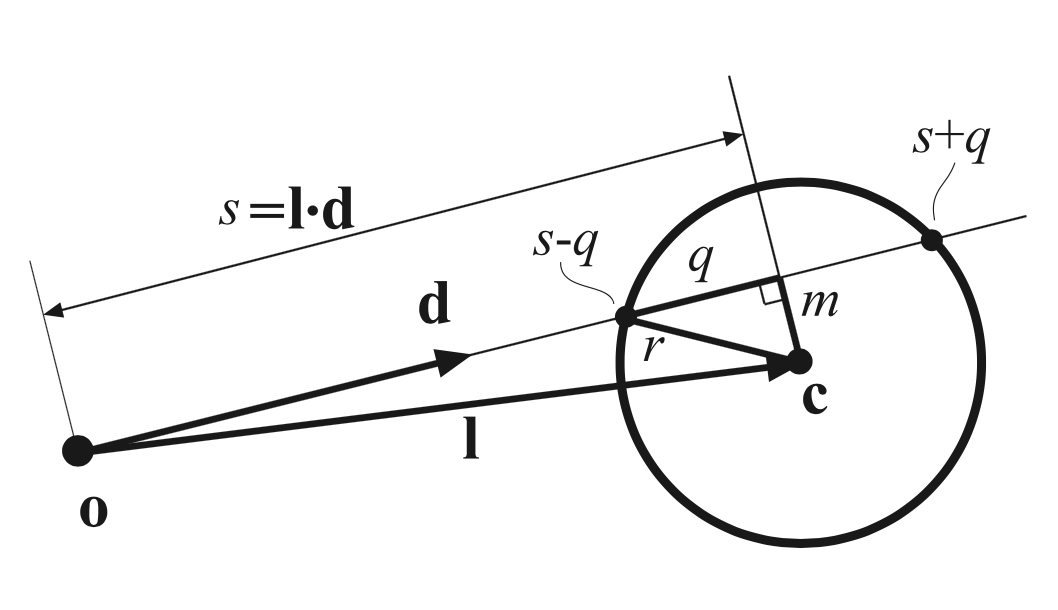
\includegraphics[width=0.4\textwidth]{ray_sphere}
    \caption{A graphical motivation for the ray-sphere intersection test}
    \label{fig:raysphere}
\end{wrapfigure}

% ray-sphere intersection
Figure \ref{fig:raysphere} is of graphical assistance for the algorithm's concept and the author will use the same notation as given on the figure. The goal of the algorithm is to compute the intersection point $p(s-q)$ if the point in front of the ray's origin or $p(s+q)$ if the ray's origin is inside the sphere. On the way the algorithm can terminate, if its sure, that there is no intersection point for the given ray and sphere. The algorithm can be split in three parts: \cite{realtime_ren}

% explain the ray-sphere intersection test splitting it into 3 parts 
\begin{enumerate}[1.]
\item This part is concerned with determining if a sphere is behind the ray's origin. If that is the case, one don't need to do further calculations and can exit the procedure for ray-sphere intersection. To do so first the vector $l = c - o$ and its squared length $l^2 = l \bullet l$ are computed. Further one computes the projection of $l$ onto the ray's direction $d$, $s = l \bullet d$. If $l^2 > r^2$ (the origin of the ray is outside the sphere) and $s < 0$ (ray's direction and the vector $l$ point in opposite directions) one can state, that the sphere is behind the ray's origin $\Rightarrow$ there is no intersection, else one can proceed with the second part of the algorithm.

\item This part is concerned with determining if the ray misses а sphere. Similarly as in the first part, if that is the case, one can jump out of the procedure. First a triangle with sides $\lvert l \rvert$, $s$ and $m$ is constructed. The values of $l^2$ and $s$ are already computed in the last part. One can compute $m^2 = l^2 - s \cdot s$ using the Pythagorean theorem. If $m^2 > r^2$ one can state, that the ray misses the sphere $\Rightarrow$ there is no intersection, else one can proceed with the last part of the algorithm.
	
\item In this part one computes the actual intersection point. To do so, a triangle with sides $r$, $m$ and $q$ is constructed. Using again the Pythagorean theorem, one can compute $q = \sqrt{r^2 - m^2}$. If $l^2 > r^2$ the sphere is in front of the ray, so the intersection point is $p(s-q)$, otherwise the ray's origin is inside the sphere and the closest intersection is $p(s+q)$.
\end{enumerate}

Later for shading purposes one would need to determine the surface normal $\hat{sn}$ of a sphere's intersection point $p$. That is easily done knowing the sphere's center $c$:

% find sphere's surface normal
\begin{align}
	\hat{sn} = \frac{p - c}{\lvert p - c \rvert}
\end{align}

% show sphere renderers 
\begin{figure}[h]
	\centering
	% show 10 spheres
	\begin{subfigure}{0.3\textwidth}
		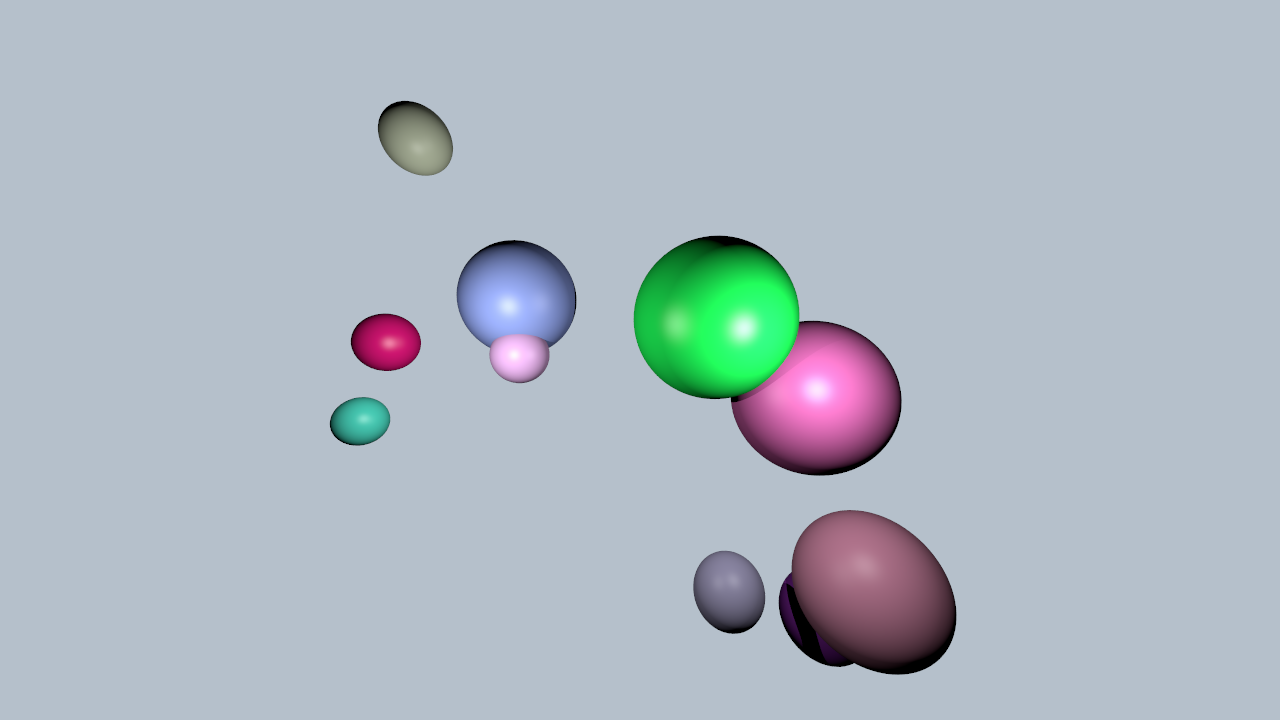
\includegraphics[width=\textwidth]{10_spheres}
		\caption{10 spheres}
		\label{fig:10spheres}
	\end{subfigure}%
	\hfill
	% show 100 spheres
	\begin{subfigure}{0.3\textwidth}
		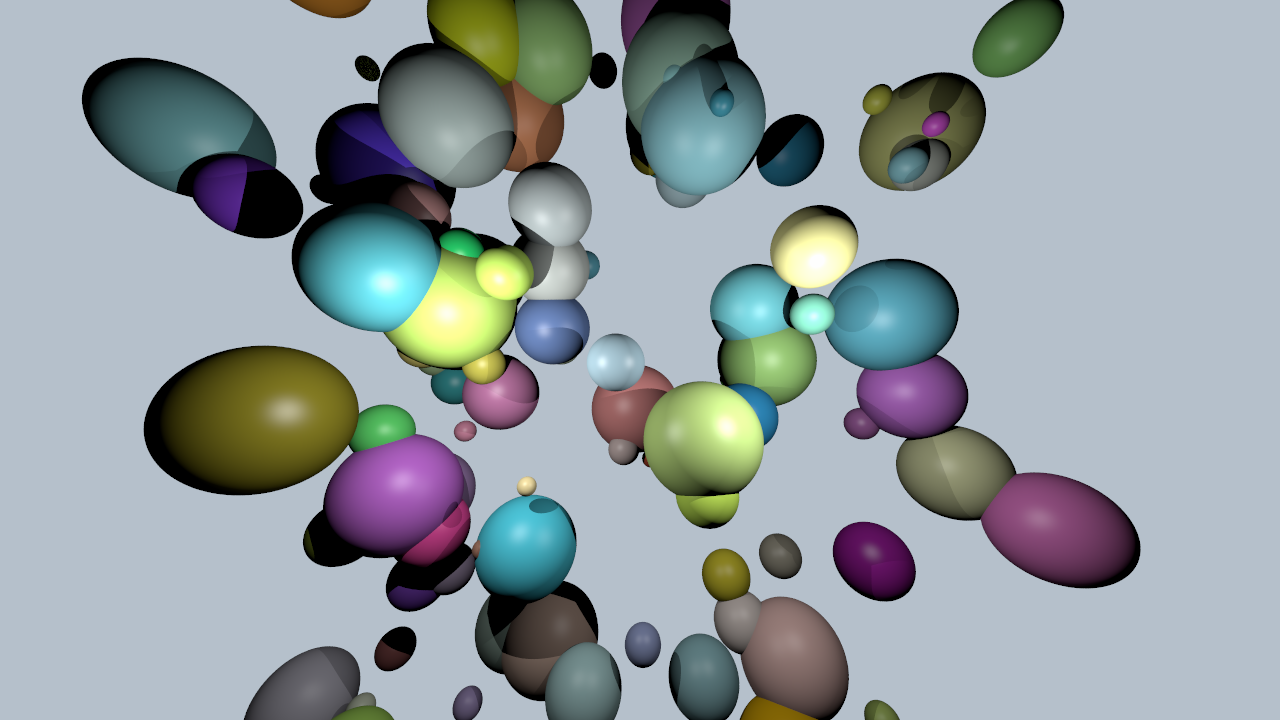
\includegraphics[width=\textwidth]{100_spheres}
		\caption{100 spheres}
		\label{fig:100spheres}
	\end{subfigure}
	\hfill
	% show 1000 spheres
	\begin{subfigure}{0.3\textwidth}
		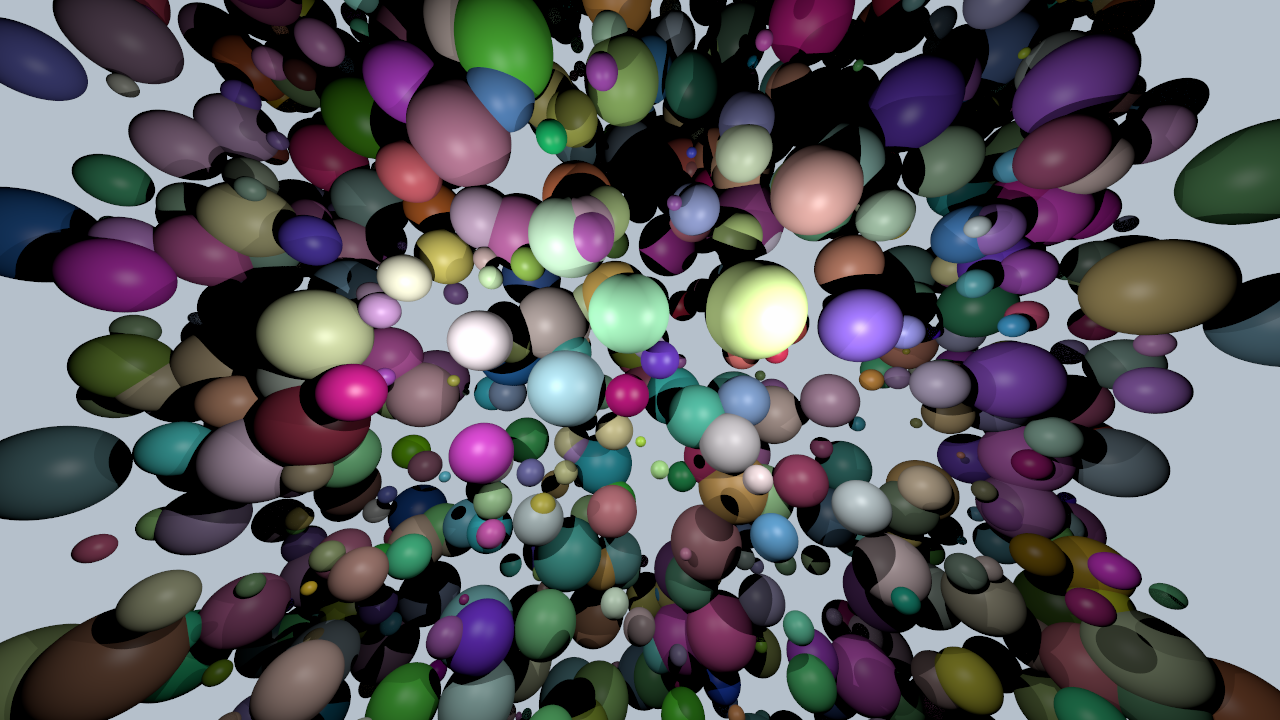
\includegraphics[width=\textwidth]{1000_spheres}
		\caption{1000 spheres}
		\label{fig:1000spheres}
	\end{subfigure}
	
	\caption{Sphere renderers}
	\label{fig:spheres}
\end{figure}

% show a table with some statistics of the renderers
\begin{table}[!ht]
\centering
	\begin{tabular}{*4c} 
		\hline
 		Characteristic & 10 spheres & 100 spheres & 1000 spheres \\ [0.5ex] 
 		\hline\hline
 		primary rays & \multicolumn{3}{c}{14,745,600} \\ 
 		shadow rays & 2,844,918 & 11,097,272 & 23,438,134 \\
 		ray-sphere intersection tests & 175,905,180 & 2,584,287,200 & 38,183,734,000 \\
 		ray-sphere intersections & 1,885,914 & 9,110,632 & 28,189,459 \\
 		render time & 4 s & 44 s & 681 s \\
 		\hline
	\end{tabular}
\caption{Rendering information of the images at fig. \ref{fig:spheres}}
\label{table:sphere_renders}
\end{table}

% put a sketch of the scene
\begin{wrapfigure}[7]{r}{0.45\textwidth} 
    \centering
    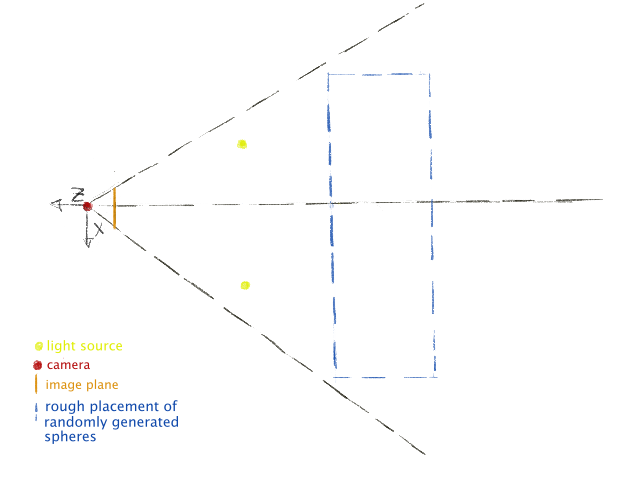
\includegraphics[width=0.45\textwidth]{sphere_scene_sketch}
    \caption{A sketch showing the scene set-up for the renderers at fig. \ref{fig:spheres}}
    \label{fig:sphere_scene_sketch}
\end{wrapfigure}

% render multiple spheres + time measurements
With the given algorithm one was able to render spheres (see figure \ref{fig:spheres}). The following renderers were done at 1280\textit{x}720 resolution with 16 samples per pixel without using any acceleration structures. For shading the Phong illumination model was used incorporating shadows as well. There are two light sources in the scene placed slightly left and slightly right in the front of the mound of spheres (see figure \ref{fig:sphere_scene_sketch}). Table \ref{table:sphere_renders} provides some rendering information. Using this initial rendering information the author was able to discover a bug, namely in the count of ray-sphere intersection tests, which values for the scenes with 100 and 1000 spheres were too close. The value for ray-sphere intersection tests for the given scenes could be easily calculated analytically:

% give the formula for the number of ray-sphere intersection tests
\centerline{\textit{ray-sphere intersection tests = (primary rays + shadow rays) * \# of spheres}}

The ray tracer used \textit{uint32\_t} ($2^{32} = 4,294,967,295$) from the standard \textit{C++} types to represent this value. Although the author was firstly unaware that this value can be easily exceeded having a big enough scene, seeing the numbers convinced him. Currently the ray tracer uses \textit{uint64\_t} to represent rendering information such as the number of ray-sphere intersection tests. \\
Making the assumption that the whole render time was spent doing ray-sphere intersections, one can give an average duration of the ray-sphere intersection test, which is roughly 20 nanoseconds. 

\subsection{Axis-aligned bounding box}

% some motivation on one why can intersect aabb
Axis-aligned bounding boxes (AABB) are used in ray tracing to bound finite objects. Ray-AABB intersections are usually faster to calculate than exact ray-object intersections, and allow the construction of bounding volume hierarchies (BVHs) which reduce the number of objects that need to be considered for each ray. \cite{aabb} \\

\vspace*{\baselineskip}

% how is a axis aligned bounding-box defined in the ray tracer
An AABB is defined in 3D space by two points: a minimum $b_{min}$ and a maximum $b_{max}$ bound. The bounds define a set of three pairs of parallel to the world coordinate axes planes, which encapsulate the box. The concept behind the ray-AABB intersection algorithm is to clip the ray by each pair of parallel planes, and if any portion of the ray remains, it intersects the AABB. The concept in 2D is illustrated by the following figure \ref{fig:aabb_concept}.

% show concept of AABB intersection test
\begin{figure}[h]
	\centering
	% show the aabb defined by xy-lines
	\begin{subfigure}[t]{0.21\linewidth}
		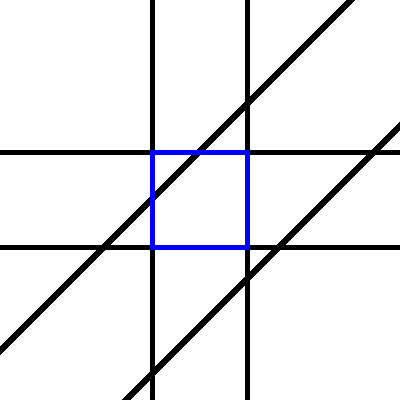
\includegraphics[width=\linewidth]{aabb1}
		\caption{The two pairs of horizontal and vertical lines define the box}
		\label{fig:aabb1}
	\end{subfigure}
\hfill
	% show the rays clipped by the x pair of lines
	\begin{subfigure}[t]{0.21\linewidth}
		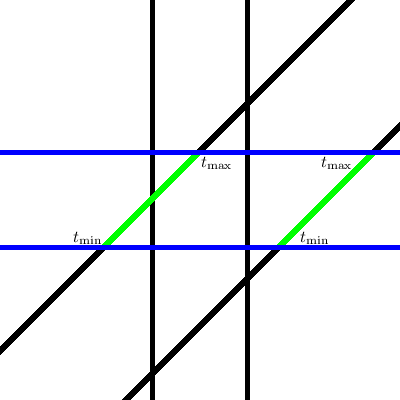
\includegraphics[width=\linewidth]{aabb2}
		\caption{The two rays are clipped by the pair of horizontal lines}
		\label{fig:aabb2}
	\end{subfigure}
\hfill
	% show the rays clipped by the y pair of lines
	\begin{subfigure}[t]{0.21\linewidth}
		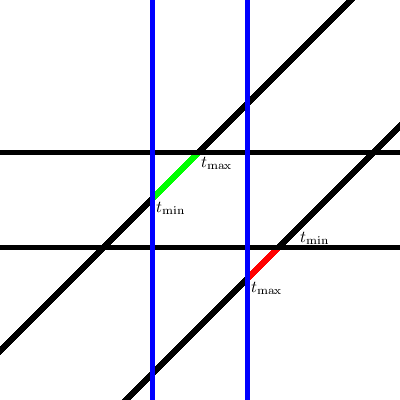
\includegraphics[width=\linewidth]{aabb3}
		\caption{The two rays are clipped by the pair of vertical lines}
		\label{fig:aabb3}
	\end{subfigure}
\hfill
	% show the remainder of the intersected ray
	\begin{subfigure}[t]{0.21\linewidth}
		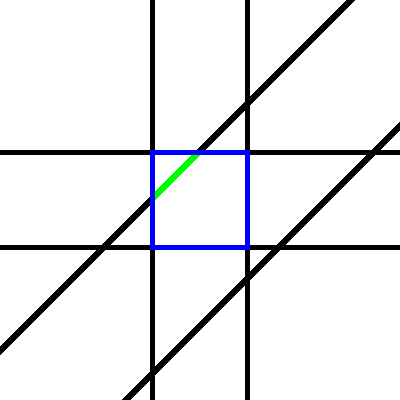
\includegraphics[width=\linewidth]{aabb4}
		\caption{The remainder of  the left ray intersects he AABB, so there is an intersection}
		\label{fig:aabb4}
	\end{subfigure}
	\caption{Concept of ray-AABB intersection test}
	\label{fig:aabb_concept}
\end{figure}

The algorithm the author used in the ray tracer is based on this concept and includes optimizations relying on IEEE numerical properties of the floating point standard that ensure the intersection test is fast and robust. This optimizations make use of the \textit{ray's inverse direction ($1 / \hat{d}$)} and \textit{ray's direction sign} data members. \cite{efficient_raybox} \\
Information about the speed gain of the render times one can achieve using AABB compared to those without would be discussed in the chapter on acceleration structures (see ch. \ref{sec:accel}). 

\subsection{Triangles}

% why does one care to intersect triangles
Triangles have become a fundamental component in many graphical applications, because of their properties (memory efficiency as triangle strip \cite{triangle_strip}, fast intersections \cite{fast_triangle_isect}, triangulation \cite{triangulation}) . In ray tracing they're naturally preferred because of these properties. Most of the \textit{state of the art} ray tracers support triangles and triangulated meshes. 

\vspace*{\baselineskip}

% show picture of the vertex order (clockwise & counter-clockwise)
\begin{wrapfigure}[10]{r}{0.45\textwidth} 
    \centering
    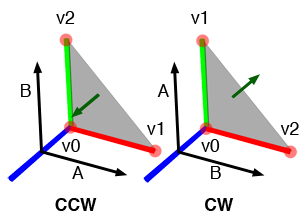
\includegraphics[width=0.45\textwidth]{triangle_vertices_n}
    \caption{The order of the vertices change the direction of the surface normal. Scratch-a-pixel%}
    \label{fig:tri_vertex_order}
\end{wrapfigure}

% how is a triangle defined in the ray-tracer
A triangle is defined by three points (called vertices) $v0$, $v1$ and $v2$ and a surface normal $n$. One important aspect of triangles, one have to keep in mind when dealing with them is the order in which the vertices are defined (clockwise or counter-clockwise), because of their order depends if the surface normal will point inwards or outwards. 

% ray-triangle intersection (geometric)

% render multiple triangles + time measurements

% how is a triangulated mesh defined in the ray-tracer

% ray-triangle intersection (MT)

% show image of rendered triangulated mesh

%----------------------------------------------------------------------------------------
%	SECTION 3
%----------------------------------------------------------------------------------------

\section{Cameras and the image plane}
\label{sec:cameras}

%----------------------------------------------------------------------------------------
%	SECTION 4
%----------------------------------------------------------------------------------------

\section{Shading}
\label{sec:shading}

%----------------------------------------------------------------------------------------
%	SECTION 5
%----------------------------------------------------------------------------------------

\section{Transformations}
\label{sec:transform}

%----------------------------------------------------------------------------------------
%	SECTION 6
%----------------------------------------------------------------------------------------

\section{Acceleration structures}
\label{sec:accel}

%----------------------------------------------------------------------------------------
%	SECTION 7
%----------------------------------------------------------------------------------------

\section{Answers to Definitions}

%----------------------------------------------------------------------------------------
%	BIBLIOGRAPHY
%----------------------------------------------------------------------------------------

\bibliographystyle{alpha}
\bibliography{references}

%----------------------------------------------------------------------------------------

\end{document}